\chapter*{Week 1: Introduction}
\addcontentsline{toc}{chapter}{Week 1: Introduction}
\setcounter{chapter}{1}
\setcounter{section}{0}

\begin{abstract}
This week you will:
\begin{enumerate}
    \item Become familiar with the Syllabus, to learn about the structure of the course and its rules and policies
    \item Install and become familiar with your Integrated Development Environment (IDE) - Visual Studio Code 
    \item Be able to identify the parts of a computer and their function in the computer system
    \item Write the "hello world" program in C++

\end{enumerate}
    
\end{abstract}

\section{Background}
This week will be an introduction to a variety of foundational material for computer science. You will need to learn how to navigate the required software, basic variables, user input, and algorithms/pseudocode. 

\subsection{Navigating Terminals and Compiling Code}
In Visual Studio Code, you can open an integrated terminal, which initially starts at the bottom of your workspace. But what is a terminal?

A \textbf{terminal} is an \textbf{interface} to your computer which allows you to execute any task on the computer directly through \textbf{commands}, without the use of a graphical user interface or GUI (like the file explorers on your system that you use to navigate to folders, create files etc). This allows you to directly execute tasks, which is often quicker than using the GUI.

VS Code has a built in terminal that you can open and use to interact with your computer's files and any code you write. To access this terminal, you will need to open VS Code. It may look like this the first time you open it:

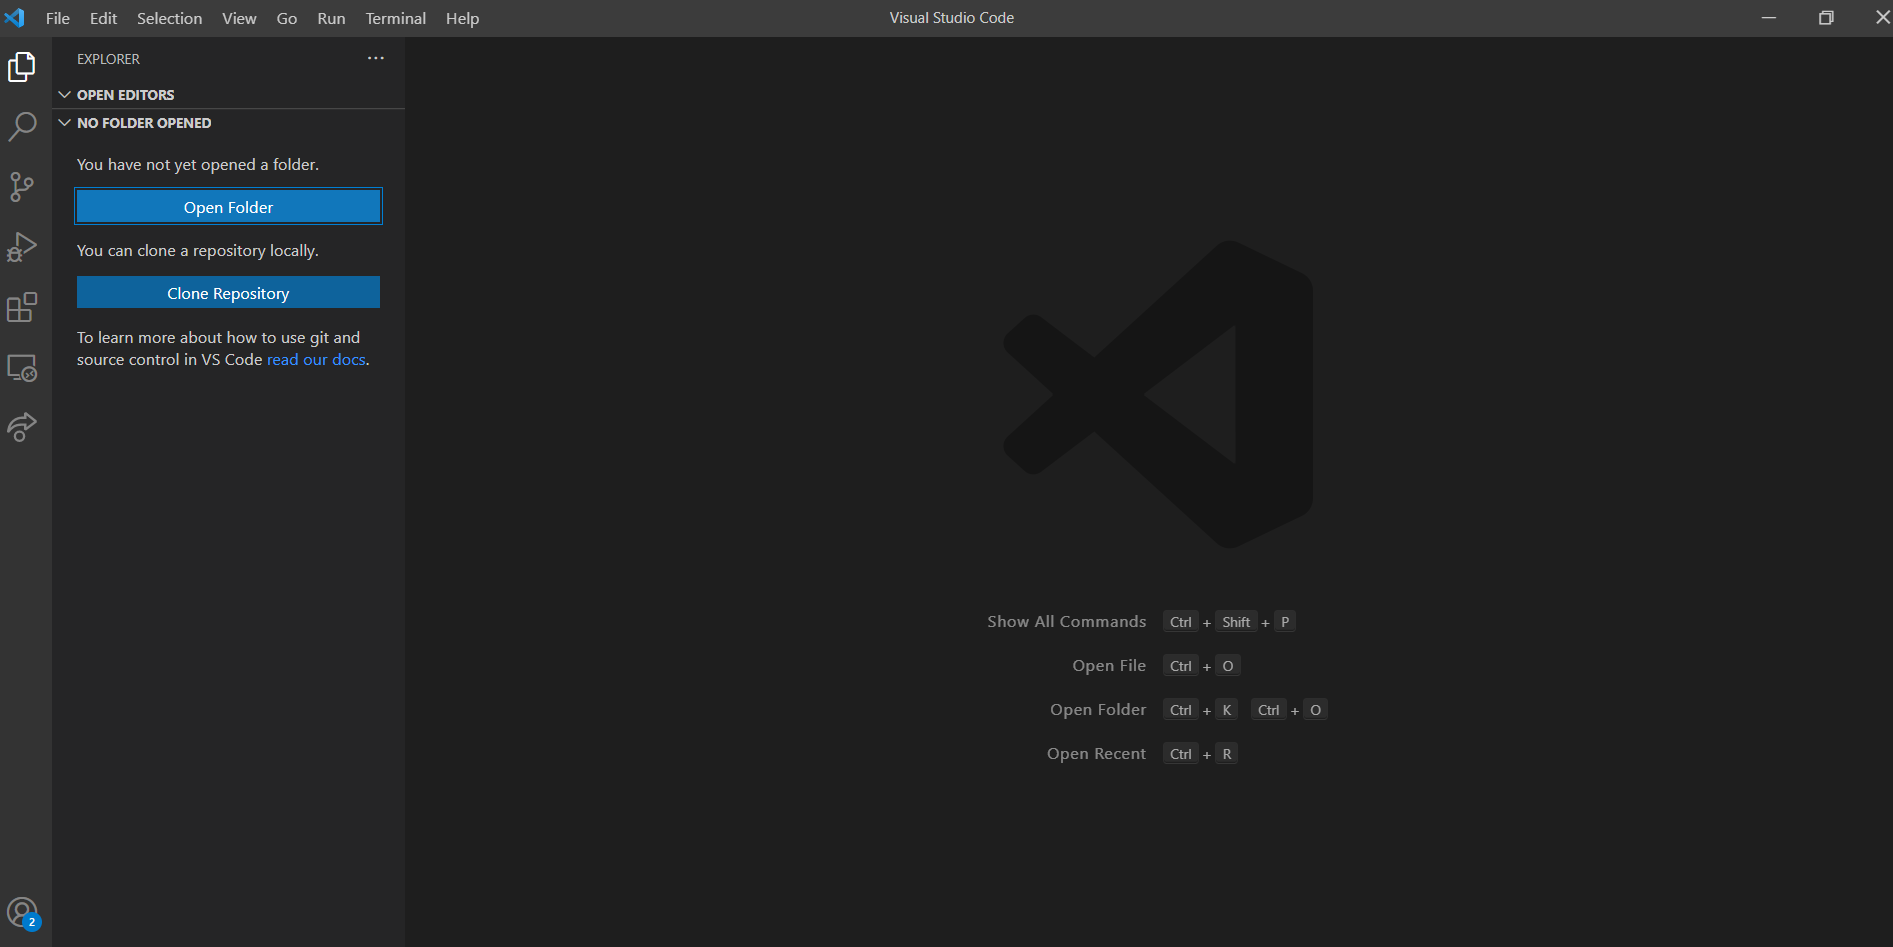
\includegraphics[width=\textwidth]{images/learn_terminal_1.png}

If you have not opened any folders yet in VS Code, you will need to start by opening one. You can do this by clicking ``Open Folder" and navigating to whichever folder you would like to use. I would encourage you to make a new folder called ``CSCI\_1300" to keep all of your course materials organized. 

Once you have a folder open, you can open a terminal. To open the Terminal tab, go to the menu bar, locate Terminal and click on it. Select ``New Terminal" to open a new terminal. A terminal looks like a dark screen when you open it and will open below the main window.

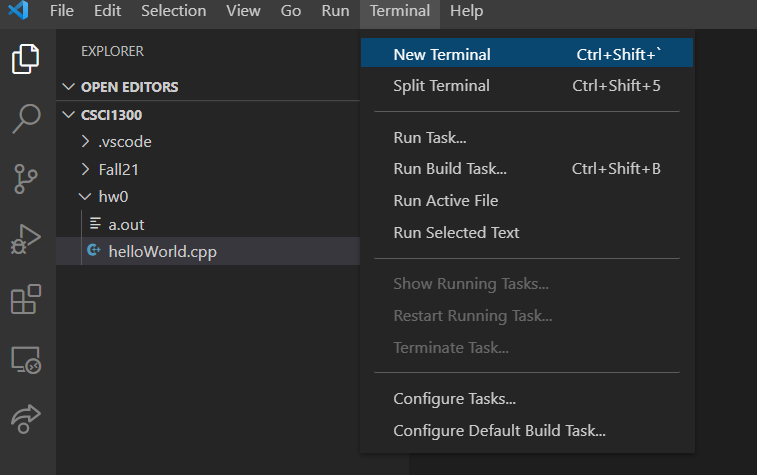
\includegraphics[width=\textwidth]{images/learn_terminal_3.png}

The new screen should look something like this: 

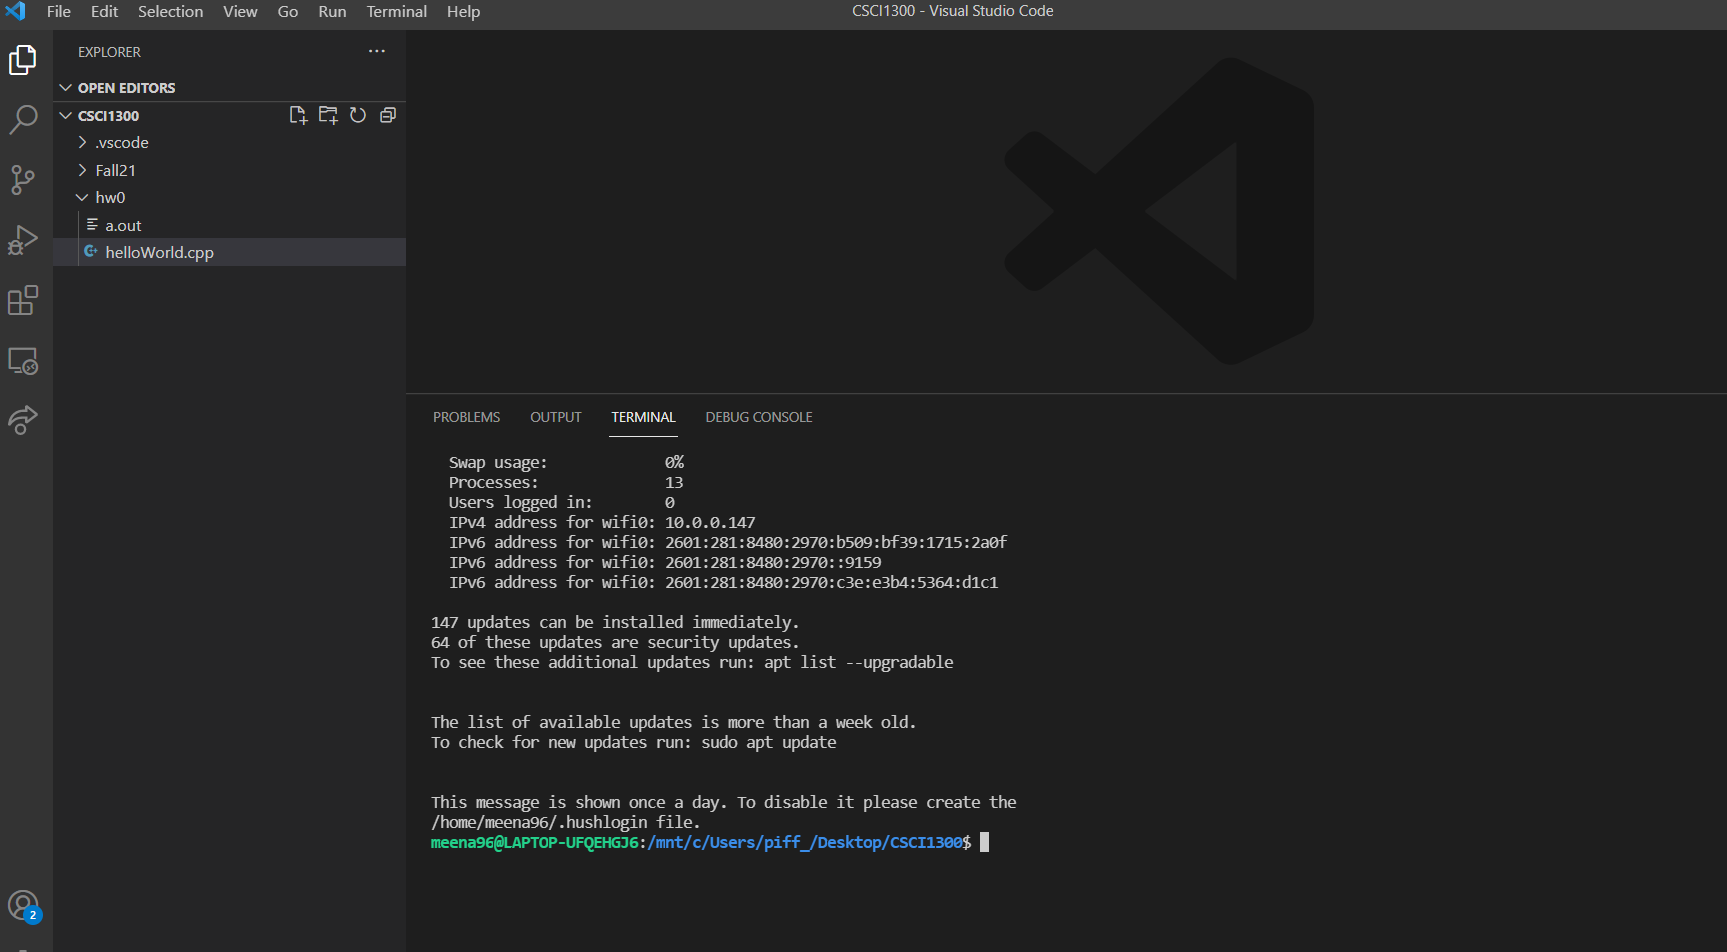
\includegraphics[width=\textwidth]{images/learn_terminal_4.png}

You will see your name and your device name on the terminal tab. Note that this can look different depending on your OS. The general anatomy of a terminal window is as follows:

\begin{enumerate}
    \item Everything before the : tells you the username and the device name where you are logged in
    \item Everything between the : and \$ is your current directory (think of a directory as the folder you’re in). Note that you do not need to be in the same directory as the screenshots shown above. Yours will depend on your computer. Mac/Linux and Windows will look different, but both will state the current directory (or ``folder") that you are in.
    \item \$ represents the end of the prompt, after which you can enter a command.
\end{enumerate}


File browsing using the terminal is like using Windows explorer/Finder or clicking on folders and navigating to different folders on your machine.

In the terminal, instead of clicking on folders we use text commands to tell the computer what we want. If we want to go to a folder where we saved our last homework, we can type the commands to navigate to that folder and display its contents.

You can read file and folder locations by their ``pathname", which is just a list of directories needed to get to your current location. Note: ``folder" and ``directory" mean the same thing, but most computer science texts will use the word ``directory". There are two different ways of expressing pathnames that you will come across; one is a constant pathname, which describes how to access a location from anywhere. A second one is a relative path name, which tells you how to get to a location from your current location. If you are already in a folder. You may see these pathnames have something like ``..", which tells the computer to go back a directory from the current location, but otherwise the style of these pathnames will look similar. 

You will need to learn the basic text commands to navigate your computer system using the terminal. Important commands to learn include how to change which folder you are in, how to see the contents of your current folder, and more. Here is a list of commands and their meanings:

\begin{table}[H]
    \begin{tabular}{p{2.5in}|p{4.0in}}
        \mintinline{bash}{ls} &  list directory contents. Note, this a lowercase l, not an uppercase ``i". This will `list' everything in the current directory. \\
        \mintinline{bash}{cd [location]} & change directory, taking you to the specified [location]. \\
        \mintinline{bash}{mkdir [name]} & make directory, which will make a new directory inside of your current location using the provided [name]. \\
        \mintinline{bash}{cp [from here] [to here]} & copy a specified file from the first specified location to the second specified location. \\
        \mintinline{bash}{mv [from here] [to here]} & move a specified file from the first specified location to the second specified location. \\
        \mintinline{bash}{zip [zip file] [listed files]} & Zip all listed files into a new zip file called [zip file]. \\
        \mintinline{bash}{rm [file name]} & permanently delete the file called [file name].
    \end{tabular}
\end{table}

Note, the square brackets are not part of the command but only to illustrate where you should insert some other text.

Finally, you will need to know how to compile code from your terminal. Let us say that we have some code in a file called ``helloWorld.cpp". In order to compile this program, we would have to navigate to the directory containing this file. Once there, you will enter the command:

\begin{minted}{bash}
        g++ -std=c++17 helloWorld.cpp 
\end{minted}

\mintinline{bash}{g++} is the compiler program.

\mintinline{bash}{-std=c++17} is the version of C++ we want to use.

\mintinline{bash}{helloWorld.cpp} is the file we wish to compile.

This command creates a file named a.out which is the compiled version of the code in helloWorld.cpp, which can be executed. You can run this compiled code using the following command:

\begin{minted}{bash}
        ./a.out
\end{minted}

Additionally, you should begin compiling with flags that tell you more information about possible errors in your code. These flags include:

\mintinline{bash}{-Wall}

Wall is short for "Warn All", which will turn on most of the warnings in C++. This will help identify various possible ways your code might go wrong, including array bounds errors and other helpful messages.

\mintinline{bash}{-Werror}

Werror will treat all warnings as errors. This will prevent you from skipping past the possible sources of error in your code, and you will need to make sure all warnings are resolved prior to compiling.

\mintinline{bash}{-Wpedantic}

This flag enables warnings that alert you about language constructs that are not ISO C or ISO C++ standard compliant. This is particularly helpful to identify constructs that may not be uniform in other compilers, which could cause problems with your code on other machines. This will help prevent instances where your code works on your personal computer, but does not work on CodeRunner or on the grader's computer. All together, your command line prompt will look something like this:

\mintinline{bash}{g++ -Wall -Werror -Wpedantic -std=c++17 myCodeFile.cpp}

Pro Tips:
\begin{itemize}
    \item Tab Complete: if you're typing something in the command line that’s very long, but unique, you can hit tab when you're partially through and it will try to fill in the rest (kind of like autocomplete). If it doesn't, and you press tab twice, it tells you everything it has as options.
    \item Command history browsing: if you have typed a command and want to repeat it, just press the up arrow. It will bring up your last executed command. Pressing up again will go to the one before. Pressing down will go forward in time through the list.
\end{itemize}

\subsection{Anatomy of a C++ Program}

You will need a couple of components for the computer to be able to understand how to translate code that you can read into something it can actually do. 

Here is a snapshot of a basic ``Hello World" program from the course textbook,  Brief C++: Late Objects, Enhanced eText. 

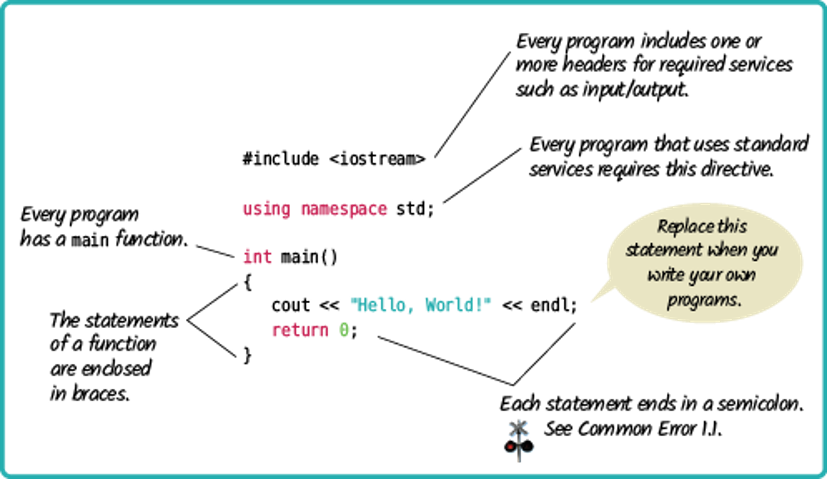
\includegraphics[width=\textwidth]{images/hello_world_16.png}

\section{Recitation}
\subsection{Software Setup}
You will need to install and become familiar with the software we will be using this semester. Follow the appropriate installation guides in Appendix A for your particular computer (Windows or Mac) to install VS Code. 

Once you have installed your software you will need to open VS Code and open the terminal. You will need VS Code and a working terminal. Take a screenshot and submit it on Canvas for this week's Recitation assignment. 

\section{Homework}

\subsection{Hello World}

%TO-DO: Update this assignment to be more clear for what files the students should make and how to zip them together

The ``Hello, World!" program is one of the simplest programs in a programming language, and it is often used to illustrate the basic syntax of a programming language. We will need to first create a folder to store our program file in and then create the file to write the program.

First, open VS Code. You can make a new folder by clicking this button: 

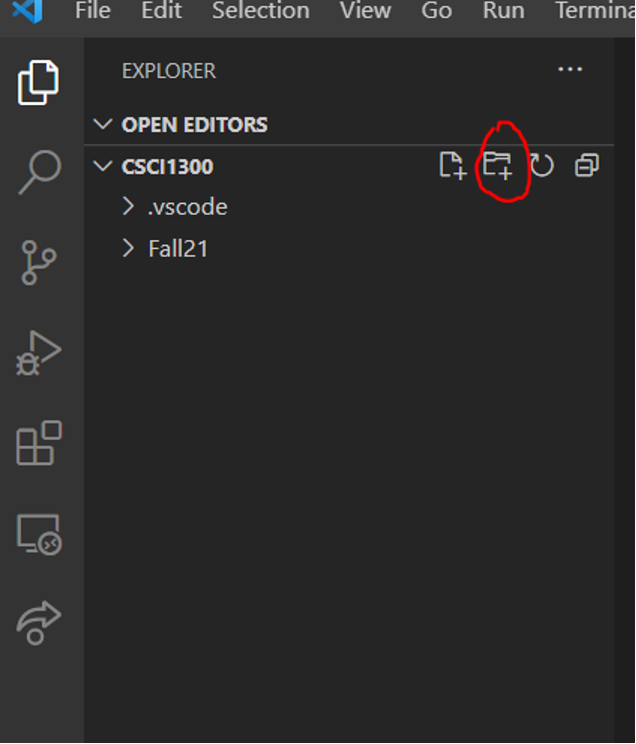
\includegraphics[width=7cm]{images/hello_world_2.png}

Name the folder something intuitive, like ``Week\_1", ``Recitation\_1", or similar. Once you have your folder you will need to create a file within it, which you can do with the toolbar across the top:

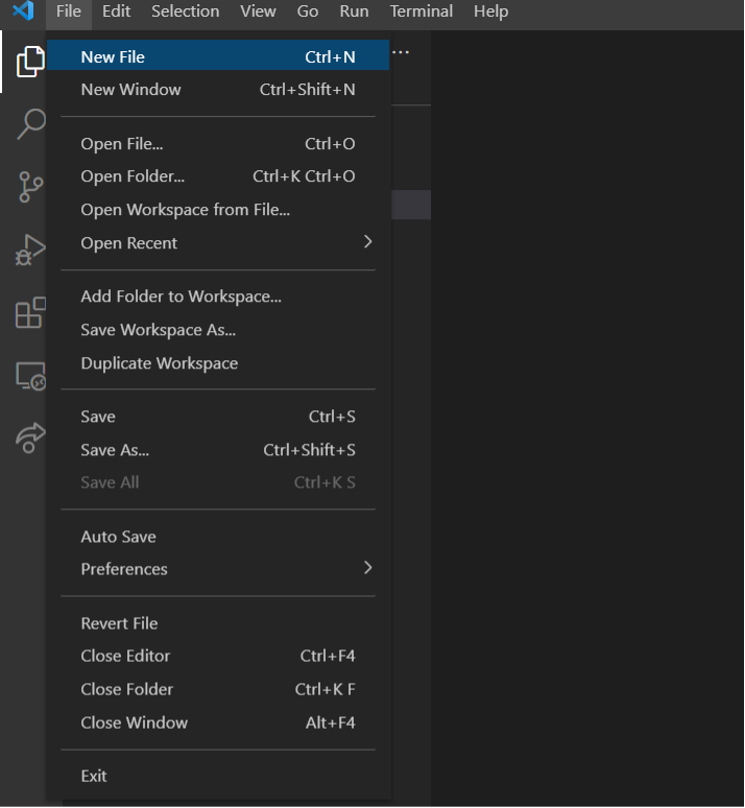
\includegraphics[width=7cm]{images/hello_world_4.png}

You should name your file \mintinline{c++}{helloWorld.cpp} -- this file name structure is important. Files of uncompiled C++ code should end with \mintinline{c++}{.cpp}, and the usage of a capital letter at the beginning of each word makes it legible even without spaces or punctuation. This style of writing names is often called ``camel case". 

Type the following code into your file:

\begin{minted}{c++}
    #include <iostream>

    int main() {
        std::cout << "Hello, world!" << std::endl;
    }
\end{minted}

Save your file.  A quick shortcut to save is Cmd + S (In Mac) or Ctrl + S (in Windows). Now you will need to compile and run your program. You can review the background information to see how to do this. Once you have completed this and successfully run your program, take a screenshot of your VS Code window including both the file and the terminal. 

\subsection{Hello World: Improved}

Now, let us explore this program a little more. Add a statement to use the standard namespace. Insert \mintinline{c++}{using namespace std;} at the beginning of the code, then we can remove the \mintinline{c++}{std::} prefixes. Your new code should look like this:

\begin{minted}{c++}
    #include <iostream>

    using namespace std;
    
    int main() {
        cout << "Hello, world!" << endl;
    }
\end{minted}

Run the program again using the steps above. Take an additional screenshot.

\subsection{Hello CSCI 1300!}

Let’s modify the file from Recitation to print ``Hello world! Hello CSCI 1300”. The text inside of the quotation marks is printed as it is. It’s case sensitive too! To see the updated output, compile and run again.

\begin{minted}{c++}
    #include <iostream>

    using namespace std;
    
    int main() {
        cout << "Hello, world! Hello CSCI 1300" << endl;
    }
\end{minted}

Once again, take a screenshot. For this section you should have three screenshots for the different Hello World programs.

Create a ZIP file that contains these three screenshots, and the three .cpp files you created, and submit it on Canvas.




